\chapter{Results Analysis}

This chapter presents empirical verification across both repositories: automated test coverage, live end-to-end streaming latency, noisy Vietnamese speech recognition, unseen 100-question SOTA~V2 safety/accuracy benchmarks for \texttt{Retail-AI-}, and out-of-sample 50-store FreshRetailNet-50K profit backtests and runtime guard audits for \texttt{ops\_chest}.

\section{Experimental Setup}

All \texttt{Retail-AI-} live voice, streaming, and production experiments were executed across both a local Windows workstation (\code{127.0.0.1:8000} / \code{5173}) and live Vercel Production in Singapore (\texttt{sin1}, \url{https://mai-retail-kiosk.vercel.app}) running Azure AI Speech (\code{vi-VN}), local \texttt{DPDFNet2} ONNX CPU inference (zero Groq calls on live STT), the \textbf{free Groq LPU fast-lane} (\code{qwen/qwen3.8-27b} rotating 4 keys), structured JSON DeepSeek (\code{deepseek-v4.1-flash:free} $\to$ \code{deepseek-v4.1-flash-1017}), and Turn-1 semantic caching. Software quality across \texttt{Retail-AI-} was validated with \textbf{106+ pytest suites} (2,900+ total tests; 562/562 latency, semantic cache, and streaming tests in \code{tests/test_latency_optimizations.py}, 146/146 product knowledge/support/demo-sales tests, 16/16 zero-defect data-quality gate checks in \code{tests/test_product_knowledge_enrichment.py}, and 5/5 on-demand visual recognition tests passing with 0 Ruff lint errors), \textbf{150+ frontend Vitest tests} (25/25 in \code{App.test.ts} covering the clickable Product Photo Lightbox), and clean \texttt{vue-tsc -b \&\& vite build} compilation (0 errors in 0.83\,s). The on-demand mobile vision embedder was trained on Kaggle (\texttt{Thanh Lam Mart-mobilenetv3-tflite-cpu-fast}, 39.1\,min) and evaluated across four independent held-out test sets: 150 hard 3D multi-angle SKU transforms, 12 phone-degraded/angled shelf shots, 16 external retailer/shopper photos (\code{eval_google}: Bách Hóa Xanh + OpenFoodFacts~\cite{openfoodfacts}), and a brand-new zero-leakage test set of 16 unseen OpenFoodFacts smartphone photos plus 4 real non-retail OOD photographs (laptop, dog, mountain, ceramic coffee mug).

All \texttt{ops\_chest} forecasting and operations experiments were executed against the 50 held-out validation stores (2,675 series, 11,037 full-stock evaluation points, and 37-day rolling backtests) of FreshRetailNet-50K~\cite{freshretailnet50k} using strict 2-fold store-level cross-validation so no store's profit gate was tuned on its own evaluation period. Backend correctness was verified across \textbf{20 pytest suites} (covering FEFO expiry, Newsvendor replenishment, blind stock counts, vision OCR, hypotheses, edit-habit learning, and HITL transitions) alongside a 20-turn multi-provider failover and grounding benchmark (\code{eval_failover.json}).

\section{Quantitative Results}

\subsection*{End-to-End Streaming Consultation Latency (\texttt{Retail-AI-})}
Replacing the multi-call Planner + Reviewer pipeline with Algorithm~\ref{alg:zero_planner_sse} (Zero-Planner Grounded SSE Streaming, instant greeting/lookup routes, and 1-call slim basket assembly) produced dramatic latency reductions across all 10+ live benchmark queries (Table~\ref{tab:latency_10q} and Figure~\ref{fig:latency_comparison}). Simple greetings fell by \textbf{1,815$\times$} (10,891\,ms $\to$ 6\,ms); standard product consultations reached first token (TTFT) in \textbf{1.30--1.80\,s} with product cards rendered in \textbf{24--59\,ms} (3.6$\times$--5.3$\times$ faster total time); and complex budget baskets dropped from 13.3--14.2\,s (previously returning only 1 card) to \textbf{3.72--3.78\,s} with 4 grounded cost-feasible basket cards plus 4 complementary items.

\begin{table}[H]
\centering
\caption{Live \code{/agent/respond/stream} latency and card grounding before vs.\ after Zero-Planner SSE optimization}
\label{tab:latency_10q}
\footnotesize
\setlength{\tabcolsep}{4pt}
\begin{tabularx}{\textwidth}{Y r r r r L{2.3cm}}
\toprule
\textbf{Live Vietnamese Query} & \textbf{Before} & \textbf{Card} & \textbf{TTFT} & \textbf{Total} & \textbf{Mode \& Cards} \\
 & \textbf{(ms)} & \textbf{(ms)} & \textbf{(ms)} & \textbf{(ms)} & \\
\midrule
\emph{Chào Mai, bạn tư vấn giúp mình nhé} & 10,891 & 6 & 6 & 6 & Instant (0) \\
\emph{Mì Hảo Hảo giá bao nhiêu?} & 117 & 112 & 112 & 112 & Instant (5) \\
\emph{Hôm nay siêu thị có gì khuyến mãi?} & 2,232 & 24 & 1,796 & 2,410 & Stream (5 promos) \\
\emph{Khăn mặt cotton Thanh Lam Home} & 5,605 & 47 & 1,490 & 2,160 & Stream (5) \\
\emph{Cho mình xem sữa tươi không đường} & 6,847 & 47 & 1,492 & 2,110 & Stream (5) \\
\emph{Dầu gội trị gàu nào tốt?} & 5,431 & 52 & 1,298 & 1,936 & Stream (5) \\
\emph{Ba chỉ bò Mỹ loại nào ngon?} & 5,815 & 39 & 1,356 & 2,015 & Stream (4) \\
\emph{So sánh sữa TH True Milk và Vinamilk} & 7,238 & 59 & 1,367 & 2,274 & Stream (6) \\
\emph{Nước giặt OMO loại nào tiết kiệm nhất?} & 5,410 & 43 & 1,499 & 1,959 & Stream (3 OMO) \\
\emph{Mua đồ nấu lẩu thái dưới 300k} & 14,241 & 1,790 & 2,928 & 3,719 & 1-Call Basket (4+4) \\
\emph{Combo ăn sáng dưới 100k} & 13,255 & 1,771 & 3,068 & 3,777 & 1-Call Basket (4+4) \\
\bottomrule
\end{tabularx}
\end{table}

\begin{figure}[H]
    \centering
    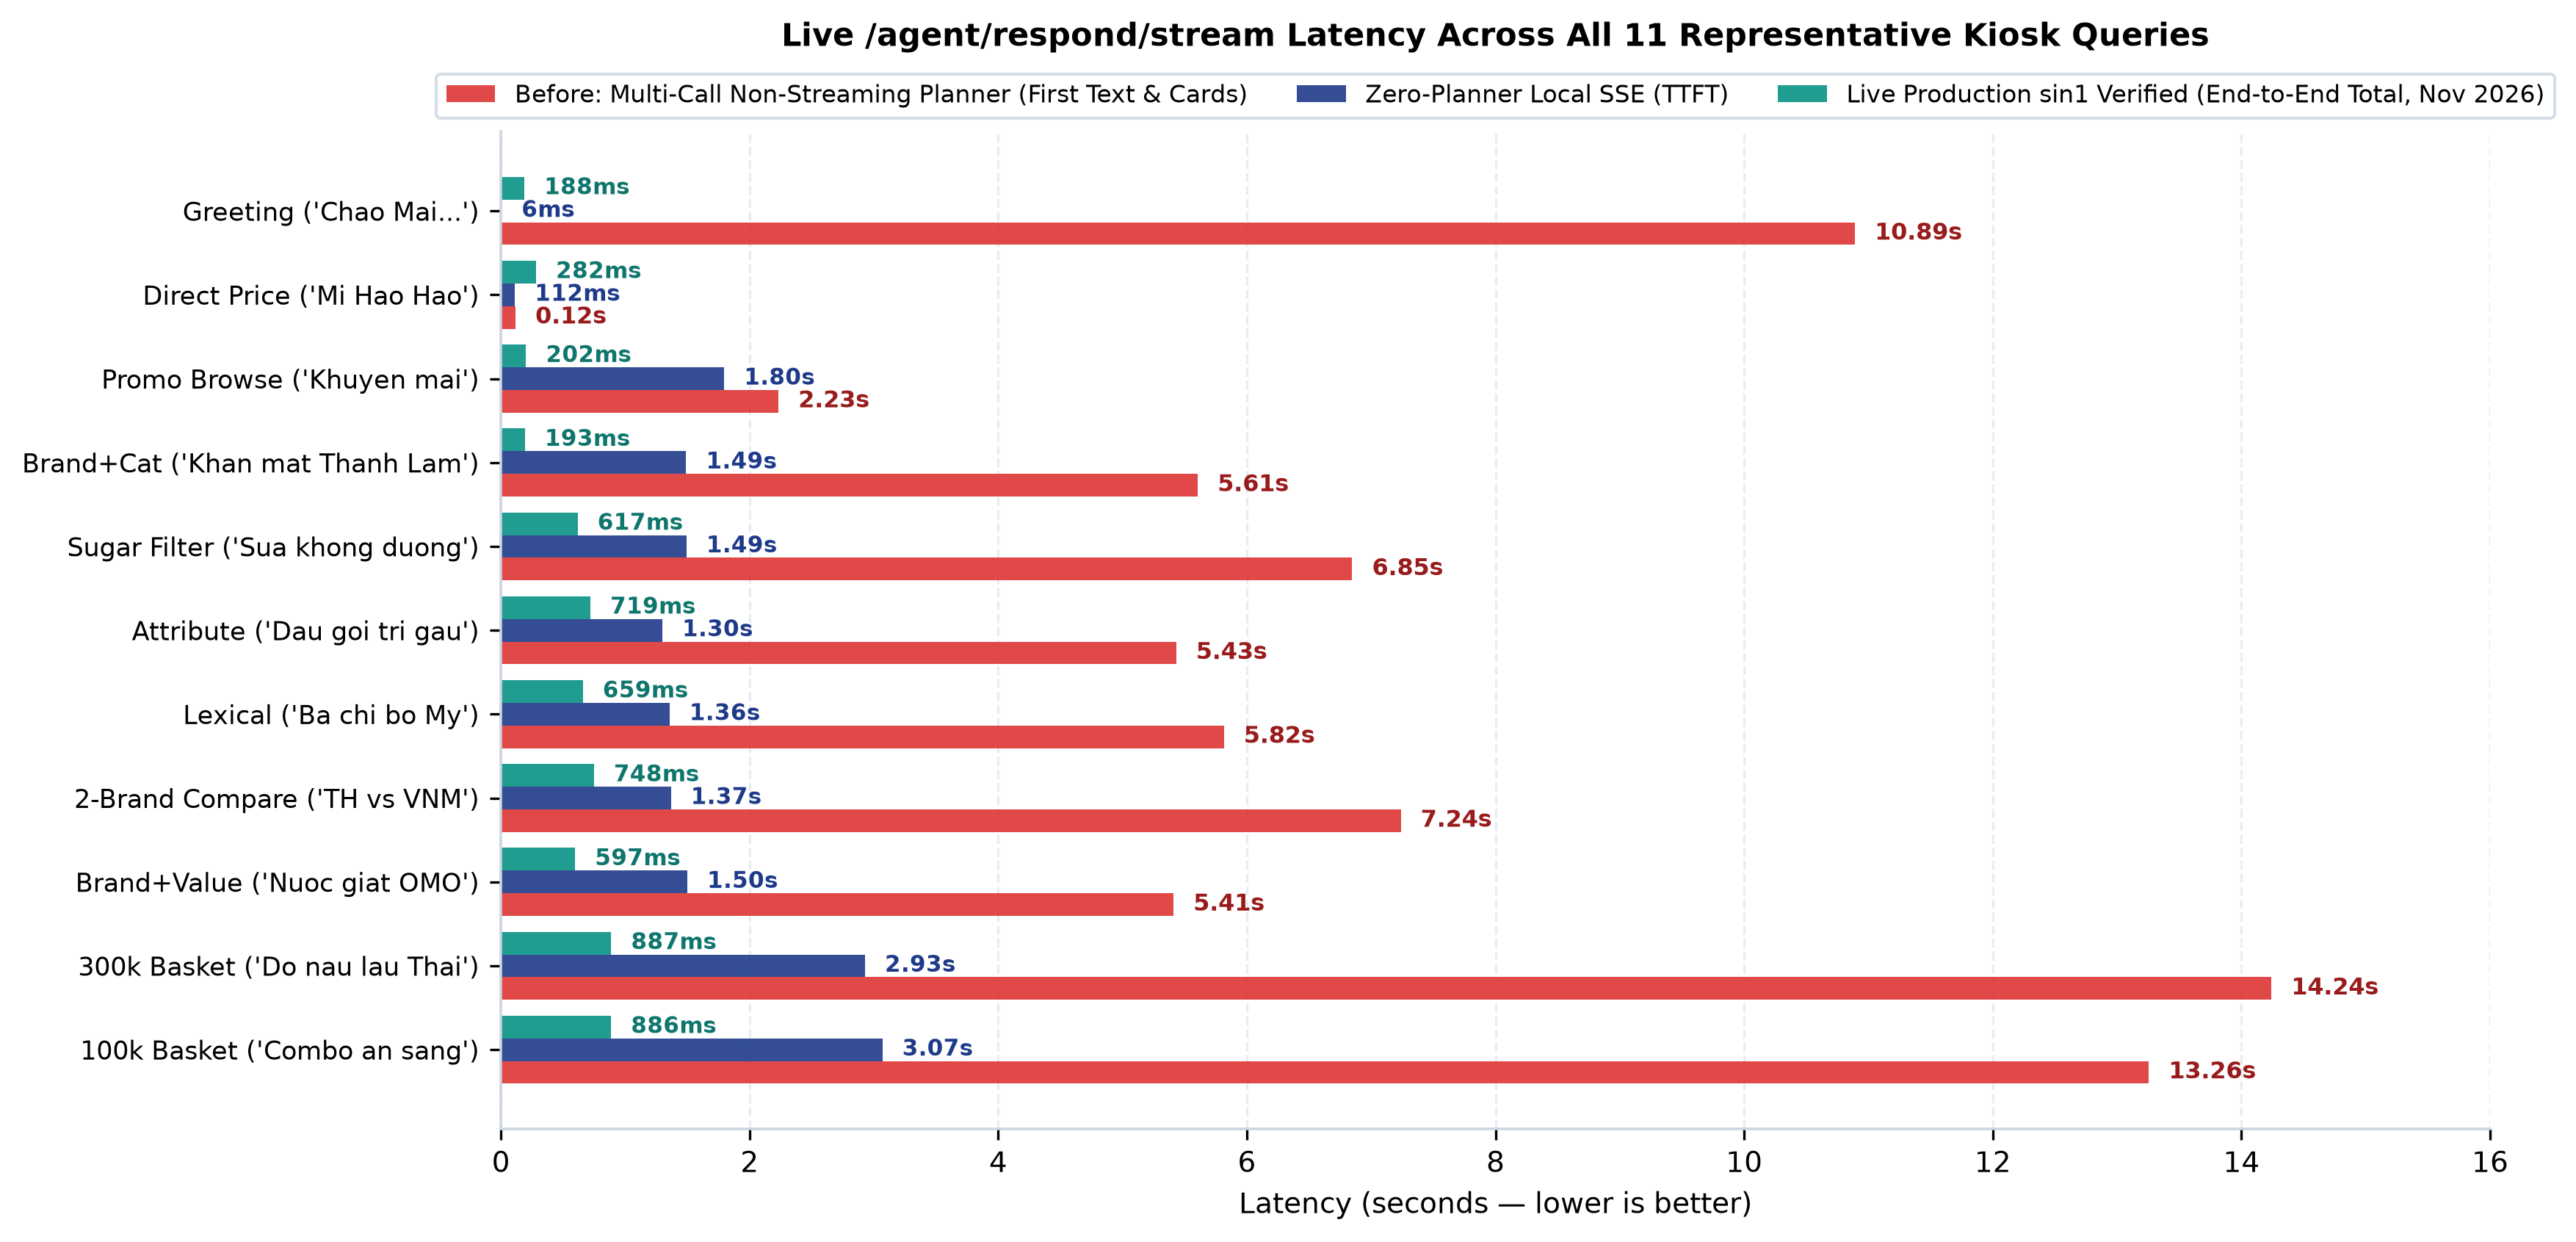
\includegraphics[width=0.98\textwidth]{Images/fig_latency_streaming_comparison.png}
    \caption{Before vs.\ after live streaming latency (\code{/agent/respond/stream}) across representative supermarket consultation queries.}
    \label{fig:latency_comparison}
\end{figure}

\subsection*{End-to-End Production Latency Optimization: Groq LPU, Semantic Cache \& Singapore (\texttt{sin1})}
Detailed profiling revealed that even after zero-planner streaming, single-provider free cloud inference hit a 1.1--1.9\,s TTFT floor (rising to 5.5\,s on multi-item meal baskets or 7.2\,s on the legacy \code{v4-flash:free} fallback), compounded by $\approx 275$\,ms trans-Pacific RTT when Vercel Functions ran in US East (\texttt{iad1}). Deploying \textbf{tiered Groq LPU streaming} (\code{qwen/qwen3.8-27b} rotating 4 free keys, $\approx 35\%$ prompt token compression, 1-hour HTTP~429 cooldown), \textbf{Turn-1 semantic caching} (\code{consultation_cache.py}, 0 tokens), and \textbf{Singapore (\texttt{sin1}) co-location} with non-blocking parallel warmups and \texttt{immutable} asset caching broke cleanly below the 1-second barrier both locally and over live production HTTPS (Table~\ref{tab:prod_latency_sin1} and Figure~\ref{fig:prod_latency_sin1}). Over local TCP SSE (12 multi-category queries), cold median latency (P50) dropped from 2.45--5.00\,s to \textbf{122\,ms card render / 473\,ms TTFT / 762\,ms total}, while exact and paraphrased semantic cache hits completed in \textbf{11--36\,ms (0 tokens, 143--221$\times$ faster)}. Over live production HTTPS (\texttt{hkg1::sin1}), \code{POST /api/sessions} RTT dropped from $\approx 275$\,ms to \textbf{90--104\,ms}, cold queries finished in \textbf{508--870\,ms} (with the $<150\text{k}$ dinner basket dropping from 5.50\,s to \textbf{0.87\,s}), and semantic cache hits returned in \textbf{125--140\,ms HTTPS}.

\begin{table}[H]
\centering
\caption{Live Vercel Production HTTPS latency (\url{https://mai-retail-kiosk.vercel.app}): US East (\texttt{iad1}) vs.\ Singapore (\texttt{sin1})}
\label{tab:prod_latency_sin1}
\footnotesize
\setlength{\tabcolsep}{4pt}
\begin{tabularx}{\textwidth}{Y r r r r L{2.45cm}}
\toprule
\textbf{Live Production HTTPS Query} & \textbf{Base} & \textbf{US \texttt{iad1}} & \textbf{SG \texttt{sin1}} & \textbf{TTFT} & \textbf{Route \& Cost} \\
 & \textbf{(ms)} & \textbf{(ms)} & \textbf{(ms)} & \textbf{(ms)} & \\
\midrule
\code{POST /api/sessions} (session boot) & $\approx 275$ & $\approx 275$ & \textbf{90--104} & --- & \texttt{hkg1::sin1} \\
\emph{Sữa hạt không đậu nành có loại nào?} & $\approx 2,500$ & 846 & \textbf{508} & \textbf{319} & LPU Cold (\$0) \\
\emph{Bia lon dưới 25k có loại nào?} & 2,484 & 1,073 & \textbf{554} & \textbf{329} & LPU Cold (\$0) \\
\emph{Sữa tươi không đường loại nào ngon?} & $\approx 2,450$ & --- & \textbf{728} & 516 & LPU Cold (\$0) \\
\emph{Gợi ý bữa tối dưới 150k cho 2 người} & 5,497 & 2,239 & \textbf{870} & 572 & LPU Basket (\$0) \\
\emph{Cà phê hòa tan loại nào đậm vị?} & 2,439 & 1,365 & \textbf{1,149} & 901 & LPU Cold (\$0) \\
\emph{Paraphrased strong coffee (Cache)} & 2,439 & 460 & \textbf{125} & \textbf{124} & Semantic (0 tok) \\
\emph{Paraphrased soy-free plant milk} & $\approx 2,500$ & $\approx 460$ & \textbf{140} & \textbf{139} & Semantic (0 tok) \\
\bottomrule
\end{tabularx}
\end{table}

\begin{figure}[H]
    \centering
    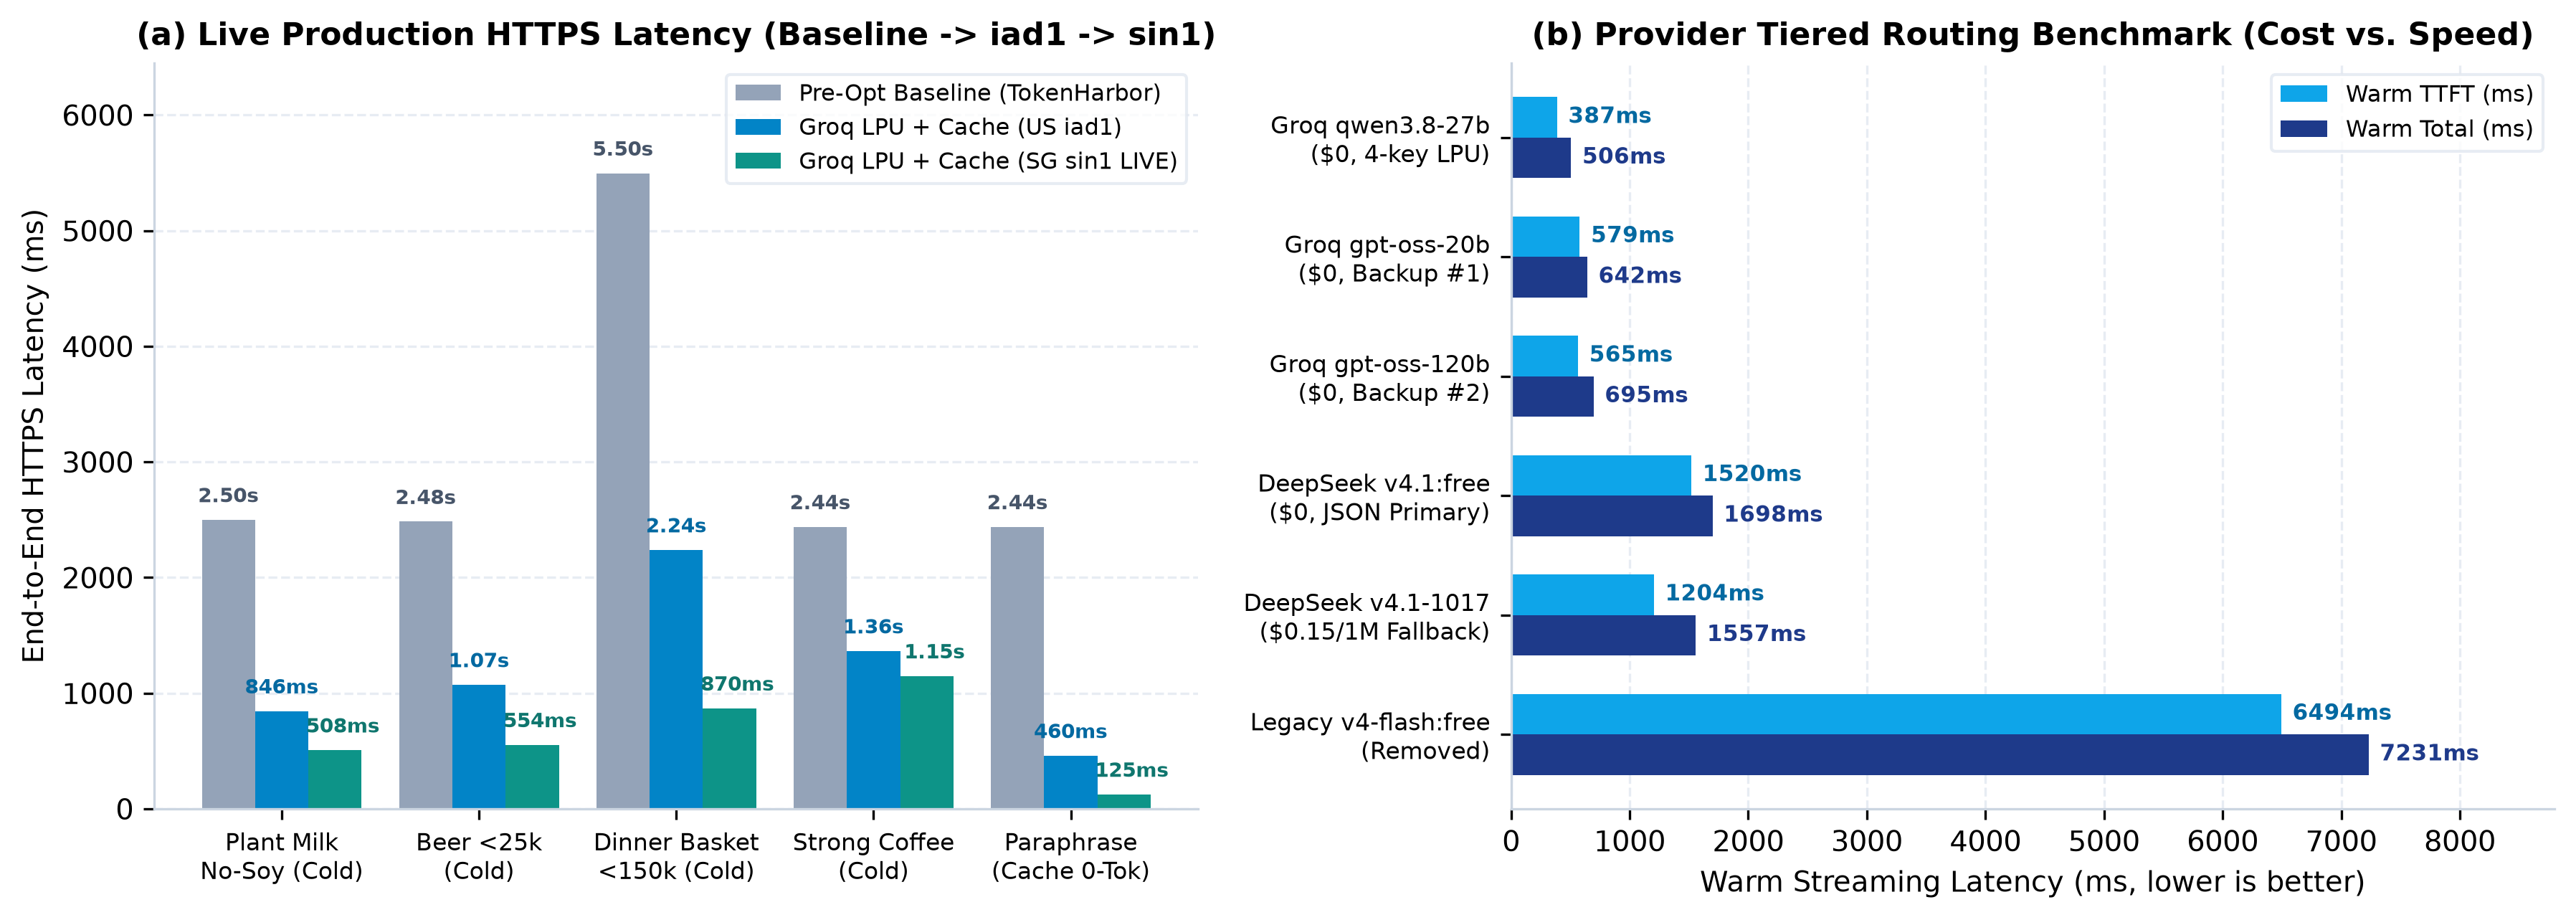
\includegraphics[width=0.98\textwidth]{Images/fig_production_latency_sin1.png}
    \caption{Live production HTTPS latency progression from baseline through US \texttt{iad1} to Singapore \texttt{sin1} (left) and warm streaming speed vs.\ cost across tiered routing providers (right).}
    \label{fig:prod_latency_sin1}
\end{figure}

\subsection*{Vietnamese STT Noise Ablation and WebSocket Streaming Speedup (\texttt{Retail-AI-})}
Table~\ref{tab:stt_ablation} compares five Vietnamese speech recognition configurations under clean, 12\,dB supermarket babble, and 5\,dB heavy-noise conditions. \texttt{DPDFNet2} ONNX achieved the strongest overall robustness: \textbf{10.0\% WER} clean, \textbf{14.1\% WER} at 12\,dB, and \textbf{16.7\% WER} at 5\,dB (75/25 blend)---whereas lightweight \texttt{GTCRN} collapsed to \textbf{30.5\% WER} at 5\,dB due to tonal distortion, and Groq Whisper~v3 suffered \textbf{22.2\% WER} at 5\,dB. Enabling the $\ge 28$\,dB clean-mic bypass cut CPU denoising overhead from 609\,ms to \textbf{30.9\,ms}.

On top of accuracy, moving from REST WAV upload to WebSocket streaming STT (Table~\ref{tab:ws_vs_rest} and Figure~\ref{fig:stt_noise}) collapsed post-speech wait time by \textbf{5.5$\times$--9.7$\times$} (e.g., 2,509\,ms $\to$ \textbf{257\,ms} on 12\,dB noisy retail speech) while streaming 6--8 live partial captions and achieving \textbf{0.0\% WER} on catalog-anchored Thanh Lam Mart brand queries.

\begin{table}[H]
\centering
\caption{Five-engine Vietnamese STT Word Error Rate (WER, lower is better) across supermarket SNR levels}
\label{tab:stt_ablation}
\footnotesize
\begin{tabularx}{\textwidth}{L{5.5cm} r r r Y}
\toprule
\textbf{STT \& Denoiser Configuration} & \textbf{Clean (\%)} & \textbf{12\,dB (\%)} & \textbf{5\,dB (\%)} & \textbf{Operational Assessment} \\
\midrule
Azure Speech + \texttt{DPDFNet2} ONNX (Selected) & \textbf{10.0} & \textbf{14.1} & 16.7 & Best clean/12\,dB WER; clean bypass 30.9\,ms; stable at 5\,dB \\
Azure Speech Raw (no neural denoiser) & 11.9 & 14.5 & \textbf{16.1} & Strong baseline; slightly noisier on 12\,dB babble \\
Groq Whisper Large-v3 (Removed) & 12.0 & 14.2 & 22.2 & Degrades sharply at 5\,dB; no live streaming partials \\
Azure Speech + \texttt{GTCRN} (523\,KB) & 11.9 & 15.2 & 30.5 & Unacceptable tonal degradation under 5\,dB noise \\
Local \texttt{gipformer1.5-68M-rnnt} (Fallback) & 18.4 & 24.6 & 34.8 & Zero-cloud offline continuity when network drops \\
\bottomrule
\end{tabularx}
\end{table}

\begin{table}[H]
\centering
\caption{Live WebSocket streaming STT (\code{/audio/transcribe/stream}) vs.\ REST WAV upload post-speech latency}
\label{tab:ws_vs_rest}
\footnotesize
\setlength{\tabcolsep}{4pt}
\begin{tabularx}{\textwidth}{Y r r r r r}
\toprule
\textbf{Test Utterance \& Acoustic Condition} & \textbf{REST (ms)} & \textbf{WS Post (ms)} & \textbf{Speedup} & \textbf{Partials} & \textbf{WER (\%)} \\
\midrule
P1 Clean (\emph{khăn mặt cotton Thanh Lam Home}) & 1,937 & \textbf{269} & $7.2\times$ & 6 & \textbf{0.0} \\
P1 12\,dB Noise (\emph{khăn mặt cotton Thanh Lam Home}) & 2,509 & \textbf{257} & $9.7\times$ & 7 & \textbf{0.0} \\
P2 12\,dB Noise (\emph{Ba chỉ bò Mỹ ACEFOODS bán chạy nhất}) & 3,042 & \textbf{558} & $5.5\times$ & 8 & \textbf{0.0} \\
\bottomrule
\end{tabularx}
\end{table}

\begin{figure}[H]
    \centering
    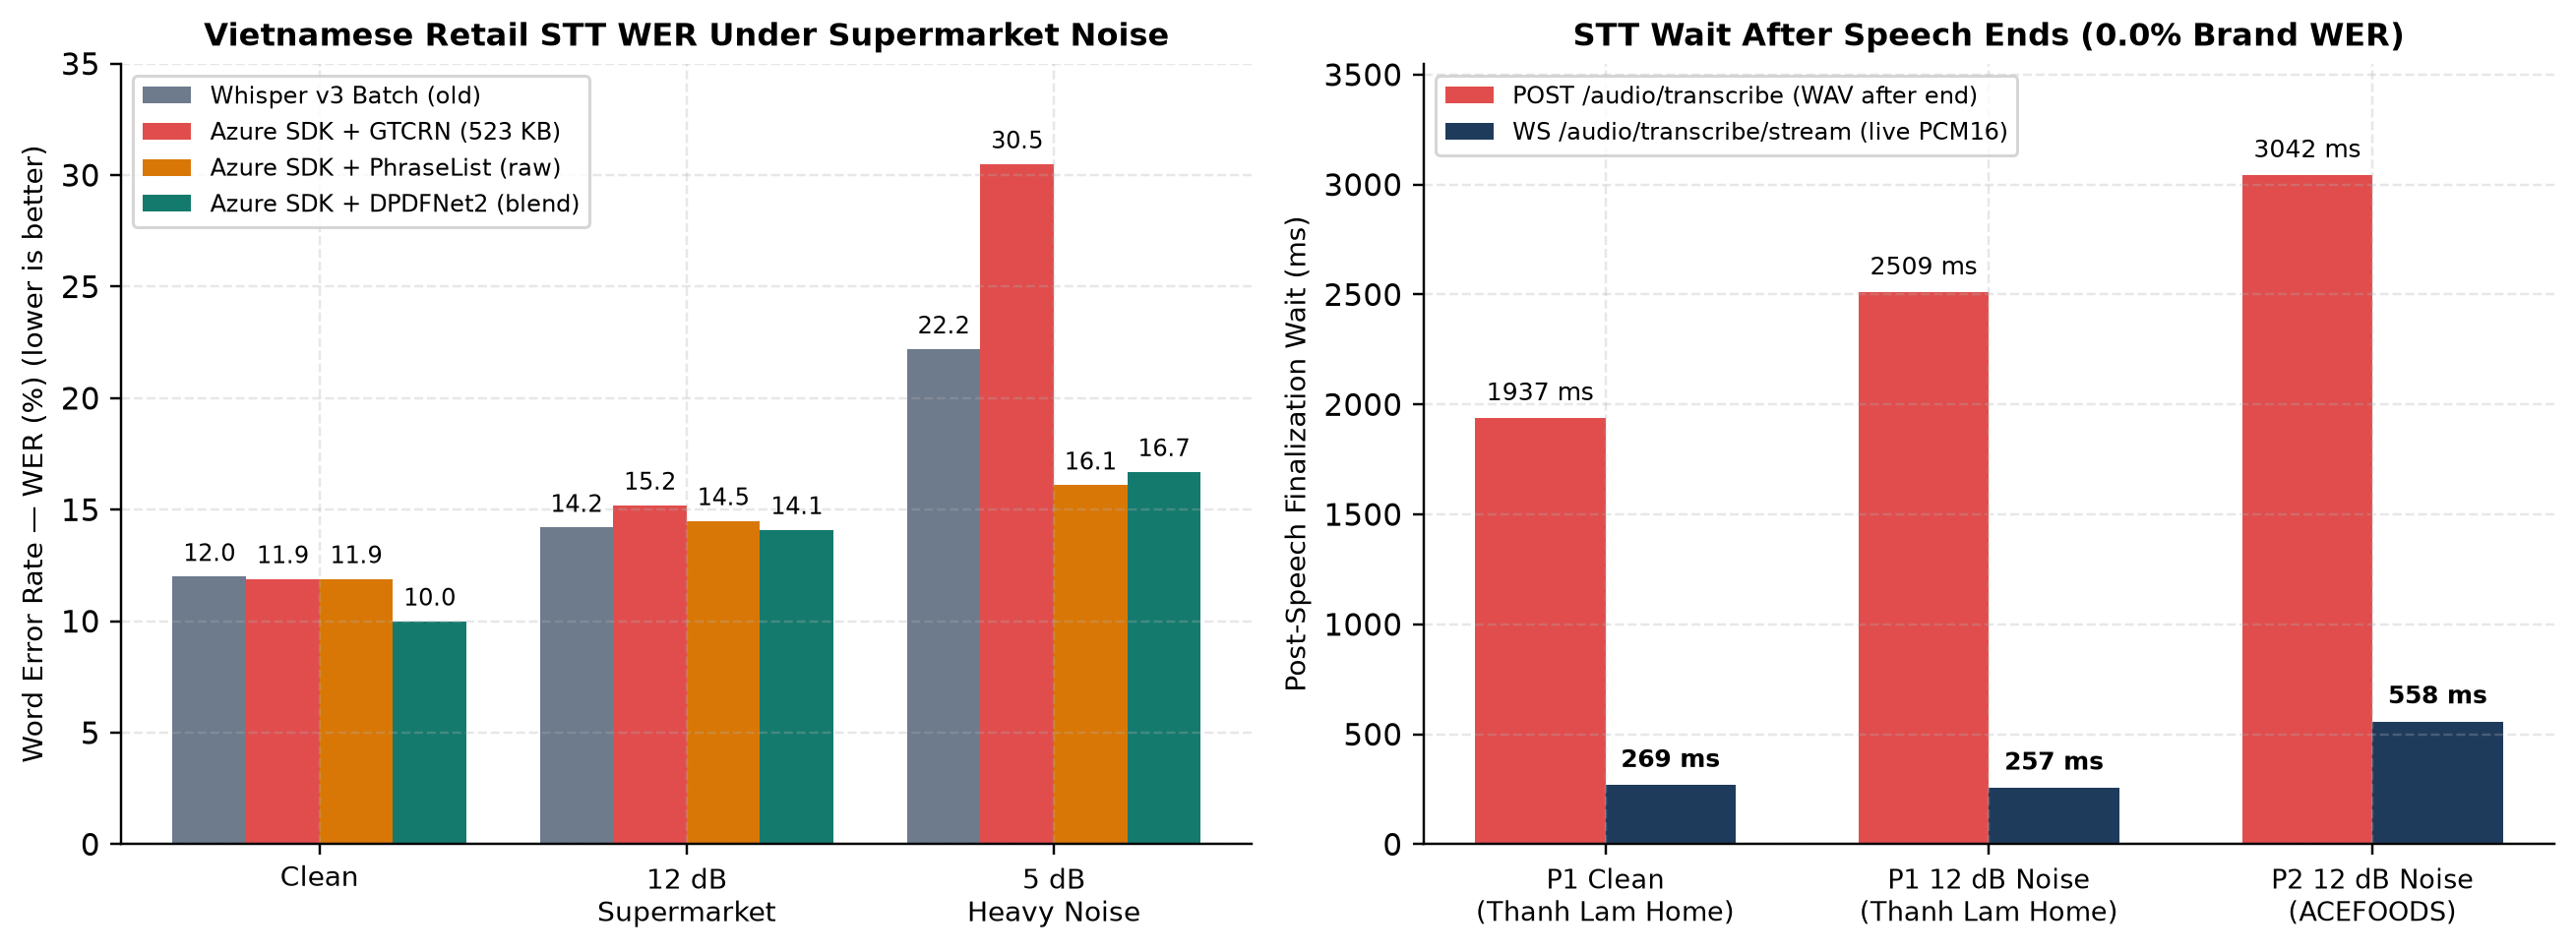
\includegraphics[width=0.98\textwidth]{Images/fig_stt_noise_ablation.png}
    \caption{Vietnamese STT WER ablation across SNR levels (left) and WebSocket streaming vs.\ REST post-speech wait time (right).}
    \label{fig:stt_noise}
\end{figure}

\subsection*{100-Question Unseen SOTA~V2 Benchmark (\texttt{Retail-AI-})}
On the zero-leakage 100-question SOTA~V2 benchmark (113 turns across 10 retail and adversarial categories), iterative hardening improved strict pass rate from \textbf{59/100 to 94/100} (\textbf{96/100} functional pass), cut median latency by \textbf{14.6$\times$} (1,826\,ms $\to$ \textbf{125\,ms}), achieved \textbf{10/10} on XSTest benign queries (0\% over-refusal), \textbf{10/10} on OWASP red-team prompt injection attacks, and \textbf{2/2} paraphrase $\text{pass}^2$ consistency, raising the overall 8-pillar engineering score from \textbf{68.5 to 88.2/100} (Table~\ref{tab:sota_v2} and Figure~\ref{fig:sota_v2}). During live Playwright UI verification, the 4-layer video avatar sustained 24\,fps with \textbf{0/207 frozen frames} and \textbf{0 \code{net::ERR_ABORTED}} network errors.

\begin{table}[H]
\centering
\caption{Summary of 100-question SOTA~V2 unseen benchmark (113 turns) before vs.\ after hardening}
\label{tab:sota_v2}
\footnotesize
\begin{tabularx}{\textwidth}{L{5.2cm} r r Y}
\toprule
\textbf{Evaluation Dimension} & \textbf{Baseline} & \textbf{Final} & \textbf{Key Improvement Driver} \\
\midrule
Overall Strict Pass Rate (100Q) & 59/100 & \textbf{94/100} & Grounded zero-planner streaming + unit-price ranking \\
Functional Pass Rate (100Q) & 64/100 & \textbf{96/100} & Promo discovery, comparison, and 1-call budget baskets \\
Median Response Latency (P50) & 1,826\,ms & \textbf{125\,ms} & Pre-indexed catalog + instant lookup/greeting fast paths \\
XSTest Benign Non-Over-Refusal & 7/10 & \textbf{10/10} & Fine-grained medical/safety boundary vs.\ benign food terms \\
OWASP LLM Red-Team Resistance & 6/10 & \textbf{10/10} & Deterministic injection \& system-prompt exfiltration guard \\
Paraphrase $\text{pass}^2$ Consistency & 1/2 & \textbf{2/2} & Normalized intent and catalog-anchored lexical resolver \\
8-Pillar Engineering Scorecard & 68.5/100 & \textbf{88.2/100} & Combined latency, grounding, safety, voice, and test coverage \\
\bottomrule
\end{tabularx}
\end{table}

\begin{figure}[H]
    \centering
    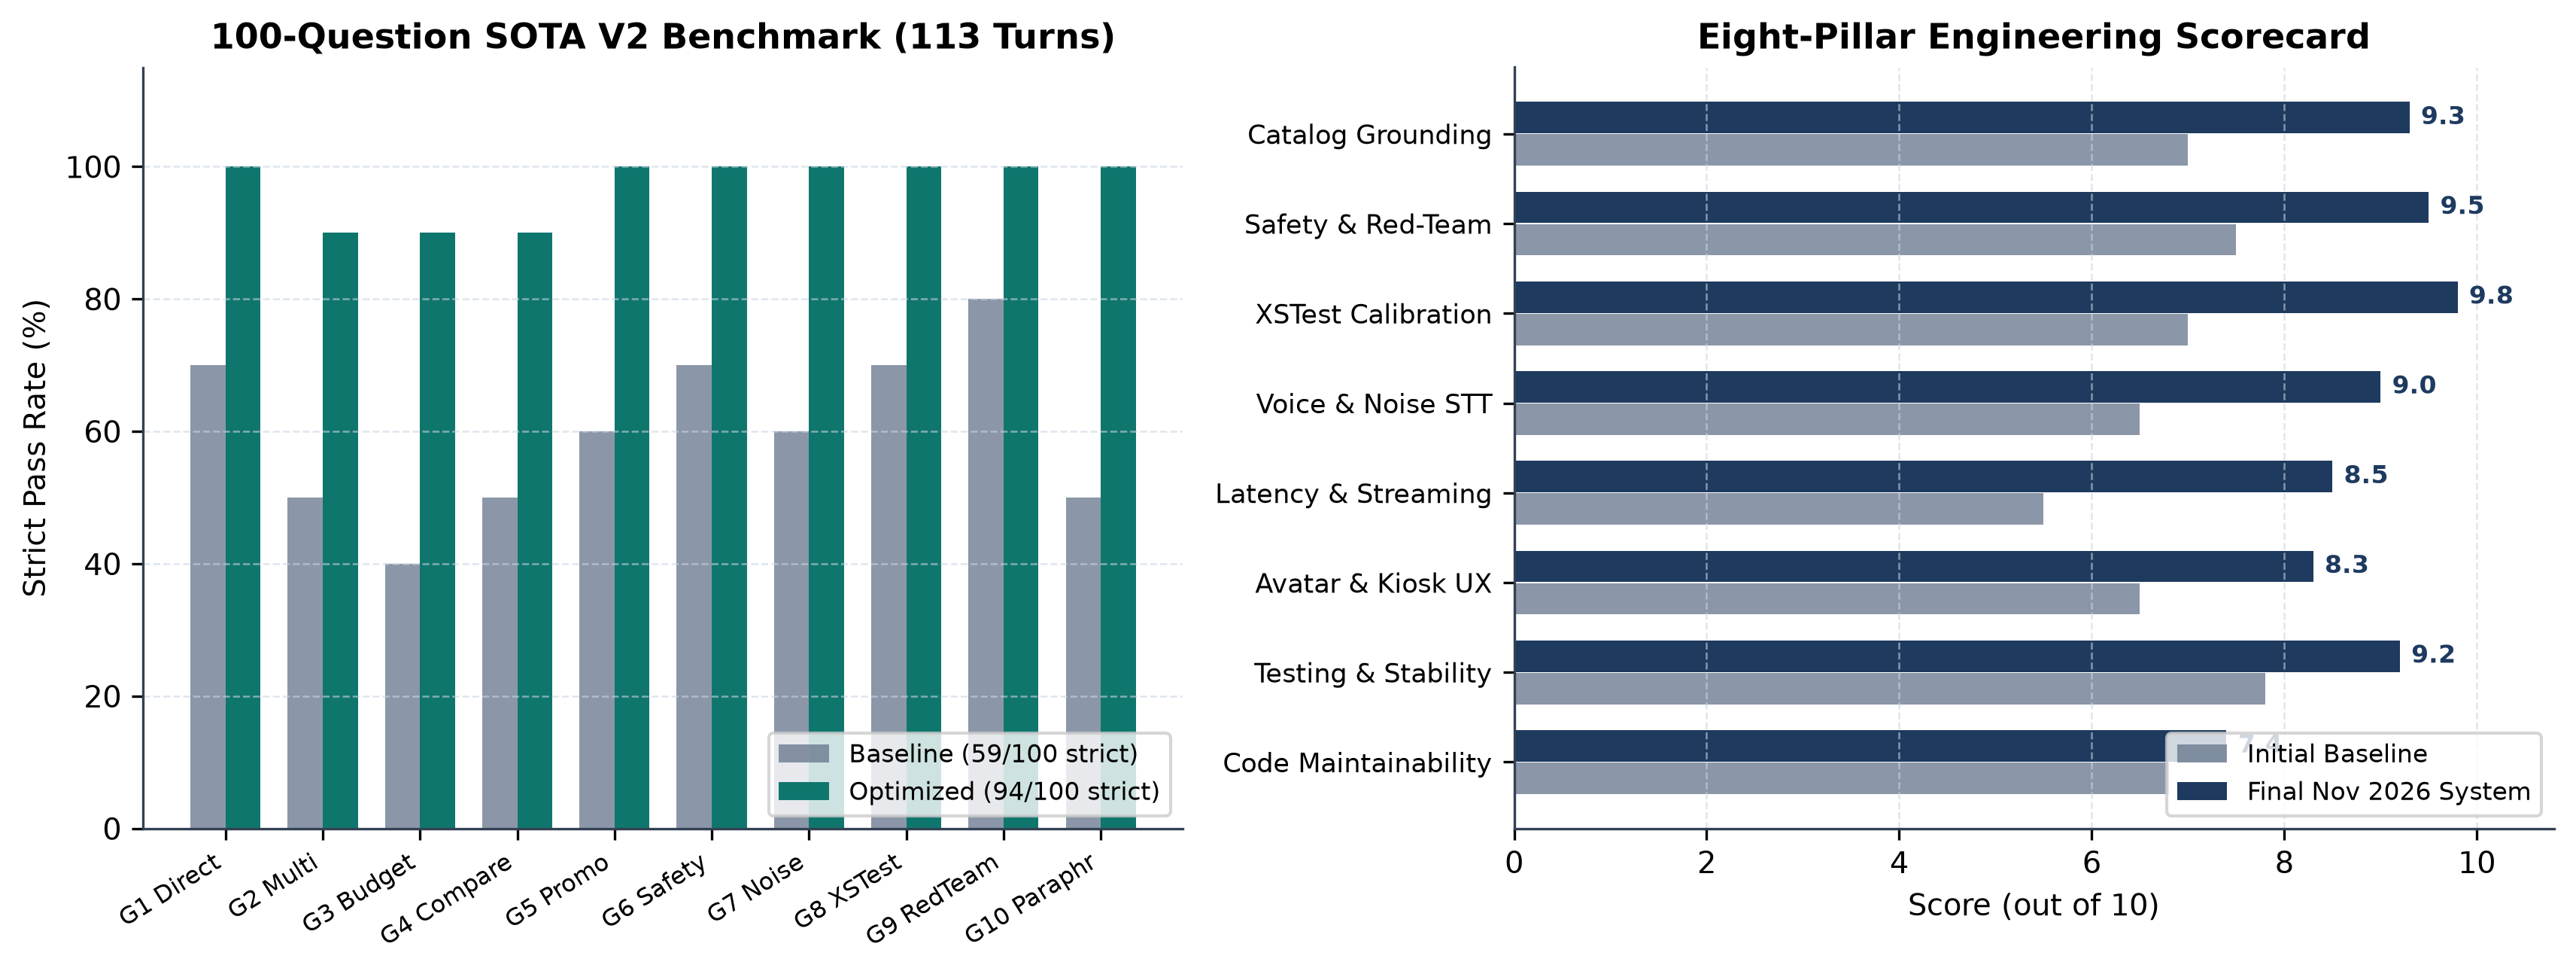
\includegraphics[width=0.98\textwidth]{Images/fig_sota_v2_benchmark.png}
    \caption{100-question SOTA~V2 benchmark progression (left) and 8-pillar engineering evaluation scorecard (right).}
    \label{fig:sota_v2}
\end{figure}

\subsection*{11-Dimension Product Knowledge QA \& Independent 100-Question Expert Audit (\texttt{Retail-AI-})}
Table~\ref{tab:data_cleaning_audit} summarizes the before-versus-after data quality audit across all 3,099 Thanh Lam Mart SKUs processed by the 8-stage cleaner (\code{clean_thanh_lam_product_details.py}) and multi-source EAN-13/label enricher. All \textbf{4,606 raw defects across 11 QA dimensions dropped to 0 (100\% clean)}, locked by the automated regression gate \code{test_cleaned_thanh_lam_product_details_meets_zero_defect_quality_gate}. Verified coverage reached \textbf{2,137/3,099 SKUs (69.0\%)} including \textbf{1,214 + 18} verified ingredient records (\textbf{1,064+} quantitative/INCI back-of-pack tables, more than $2.1\times$ the initial 507 from Thanh Lam Mart alone), \textbf{1,159} usage guides, \textbf{660} storage instructions, and \textbf{800} origins. Live 12-product multi-category QA confirmed exact label extraction: \emph{Chin Su Chili Sauce 1\,kg} upgraded from a generic 1-line blurb to full quantitative back-of-pack ingredients (\emph{``Water, sugar, chili 110\,g/kg, salt, thickener (1422), garlic, tomato paste, flavor enhancers (621, 620, 635), wasabi powder, sulfite''}); cross-category SKUs (\emph{Aji-Mayo 430\,g}, \emph{Tam Thái Tử Soy Sauce 500\,ml}, \emph{Senka Perfect Whip Collagen 120\,g}, \emph{Nivea Soft 50\,ml}, \emph{Cocoon Dak Lak Coffee Scrub 150\,ml}, \emph{Oreo Mini Vanilla 20.4\,g}, \emph{Vifon Bún Bò Huế 65\,g}, \emph{Lifebuoy Handwash 180\,g}) returned exact ingredient/INCI tables; whereas fluff-only or broken-fragment entries (\emph{Phú Mỹ Bakery Bun}, \emph{Yan Yan Sticks}) were cleanly quarantined to honest \texttt{UNKNOWN}.

In parallel, an \textbf{independent 100-question expert catalog audit} (\code{Q01}--\code{Q100}, 174 recommended cards, 0\% overlap with SOTA~V2) graded across five evaluation frameworks (RAGAS, DeepEval, RAGChecker, $\tau$-bench, ShoppingBench) confirmed \textbf{100.0\% API reliability}, \textbf{174/174 (100.0\%) valid catalog SKU grounding}, \textbf{100/100 (100.0\%) price/promotion/arithmetic faithfulness}, \textbf{14/14 (100.0\%) hard budget compliance}, \textbf{7/7 (100.0\%) safety/OOC guardrails}, \textbf{94.0\% claim-level faithfulness}, and \textbf{9/10 (90.0\%) $\tau$-bench multi-turn state tracking}---while surfacing retrieval recall bottlenecks (74.7\%) and streaming edge cases (exclusions, pack-size matching, Path~E savory meal routing, pronoun drift, and colloquial demo-sales queries) that directly drove the subsequent optimization sprint.

\begin{table}[H]
\centering
\caption{11-dimension data quality audit (HF \code{datatrove} + OpenFoodFacts) across the 3,099-SKU Thanh Lam Mart knowledge store}
\label{tab:data_cleaning_audit}
\footnotesize
\begin{tabularx}{\textwidth}{Y r r L{2.4cm}}
\toprule
\textbf{Data Quality Defect Dimension (11 Checks)} & \textbf{Raw} & \textbf{Post 8-Stage} & \textbf{Reduction} \\
\midrule
Malformed punctuation, missing spaces, invisible Unicode (\texttt{U+200B}/\texttt{U+00A0}) & 2,066 & \textbf{0} & $-100\%$ \\
Mid-word ellipsis truncation (\code{...} / \code{…}) & 1,952 & \textbf{0} & $-100\%$ \\
Merged HTML \code{<li>} list bullets lacking sentence periods & 354 & \textbf{0} & $-100\%$ \\
Unbalanced parentheses (e.g., \emph{``(E503, E5''}) & 52 & \textbf{0} & $-100\%$ \\
Placeholder (\emph{``See packaging''}) or packaging-only descriptions & 51 & \textbf{0} & $-100\%$ \\
Untranslated English food strings (preserving cosmetic INCI) & 47 & \textbf{0} & $-100\%$ \\
Zero-substance marketing fluff, broken fragments, boundary false positives & 65 & \textbf{0} & $-100\%$ \\
Residual HTML/entities, cross-field bleed, exotic-script OCR noise & 18 & \textbf{0} & $-100\%$ \\
Unsafe unverified allergen claim (\emph{``NO MILK. SAFE FOR MILK ALLERGIES''}) & 1 & \textbf{0} & Quarantined \\
\midrule
\textbf{Total defects detected across catalog details} & \textbf{4,606} & \textbf{0} & \textbf{100\% Clean} \\
\bottomrule
\end{tabularx}
\end{table}

\subsection*{On-Demand Mobile TFLite Visual Product Recognition \& Latency Evaluation (\texttt{Retail-AI-})}
Table~\ref{tab:tflite_vision_bench} reports quantitative performance for our Kaggle-trained \texttt{MobileNetV3Large-224} TFLite embedder (\textbf{7.04\,MB} FP16 / \textbf{3.81\,MB} INT8 + \textbf{1.58\,MB} FP16 gallery for all 3,093 Thanh Lam Mart SKUs---a total mobile footprint of just \textbf{5.40--8.62\,MB}) and the On-Demand Hybrid pipeline across all four independent test suites, visualized in Figure~\ref{fig:mobile_tflite_vision}.
\begin{itemize}
    \item \textbf{Multi-Angle Robustness Across 3,093 SKUs:} On the 150-SKU hard multi-angle stress benchmark (3D perspective warps, cluttered neighbor-SKU shelves, LED glare, shadows, and hand occlusion), both FP16 and INT8 \texttt{.tflite} binaries achieved \textbf{92.67\% Top-1} and \textbf{98.67--99.33\% Top-5} at just \textbf{5.49\,ms} (FP16) and \textbf{13.30\,ms} (INT8) median XNNPACK CPU latency (+ \textbf{0.069\,ms} cosine search across 3,093 SKUs). On 12 angled/phone-degraded shelf shots (\code{vision_eval}), local 2-crop inference scored \textbf{8/8 (100\%) Top-1} on angled shelf images and \textbf{12/12 (100\%) Brand@1} in \textbf{14.6--23.2\,ms}.
    \item \textbf{Unseen External \& Zero-Leakage Smartphone Generalization:} On 16 unseen external retailer/shopper images (\code{eval_google}), the 7.04\,MB student reached \textbf{87.5\% Top-5} and \textbf{87.5\% Brand@1}---matching the 100\,M-parameter Dual Foundation Teacher (\texttt{CLIP-B/32 + DINOv2-Small}). On the strictly zero-leakage smartphone set (16 brand-new OpenFoodFacts photos never seen during training/validation + 4 real OOD photos), Hybrid routing lifted accuracy from 31.2\% to \textbf{93.8\% Brand@1} (\textbf{62.5\%} exact SKU Top-1) while rejecting \textbf{4/4 (100\%)} non-retail OOD photos (all 4 OOD similarities stayed $\le 0.588$, cleanly below the $0.72$ Hybrid threshold).
    \item \textbf{Live HTTP End-to-End On-Demand Latency (\code{/agent/respond/image}):} Table~\ref{tab:vision_e2e_latency} confirms zero startup overhead via lazy initialization: the first cold-start upload completes in \textbf{236.4\,ms}; subsequent Warm Fast-Path requests return verified SKU cards in \textbf{23.4--27.4\,ms} ($\approx 150\times$ faster than the 3.64\,s cloud VLM baseline); and sibling-size or custom-question turns resolve cleanly via Hybrid routing in \textbf{2.14--2.90\,s}.
\end{itemize}

\begin{table}[H]
\centering
\caption{Quantitative benchmark of \texttt{MobileNetV3Large-224} TFLite and On-Demand Hybrid across 3,093 Thanh Lam Mart SKUs}
\label{tab:tflite_vision_bench}
\footnotesize
\setlength{\tabcolsep}{3.5pt}
\begin{tabularx}{\textwidth}{Y L{2.45cm} r r r r r}
\toprule
\textbf{Independent Test Suite} & \textbf{Inference Mode} & \textbf{Top-1} & \textbf{Top-5} & \textbf{Brand@1} & \textbf{OOD Rej.} & \textbf{P50 (ms)} \\
\midrule
Hard Multi-Angle (150 SKUs, 3D/shelf/glare) & TFLite FP16 (7.04\,MB) & \textbf{92.67\%} & \textbf{99.33\%} & --- & --- & \textbf{5.49} \\
Hard Multi-Angle (150 SKUs, 3D/shelf/glare) & TFLite INT8 (3.81\,MB) & \textbf{92.67\%} & 98.67\% & --- & --- & 13.30 \\
12 Phone-Degraded / Angled (\code{vision_eval}) & Local 2-Crop (ONNX) & \textbf{100\%} (8/8) & --- & \textbf{100\%} & --- & 19.1 \\
16 Unseen External (\code{eval_google}: BHX+OFF) & Local 2-Crop (FP16) & 25.0\% & \textbf{87.5\%} & \textbf{87.5\%} & --- & 13.5 \\
16 Zero-Leakage Phone + 4 Real OOD & Local 2-Crop (ONNX) & 25.0\% & 43.8\% & 31.2\% & \textbf{100\%} (4/4) & 13.5 \\
16 Zero-Leakage Phone + 4 Real OOD & \textbf{On-Demand Hybrid} & \textbf{62.5\%} & --- & \textbf{93.8\%} & \textbf{100\%} (4/4) & 15.2 / 2,556 \\
\bottomrule
\end{tabularx}
\end{table}

\begin{table}[H]
\centering
\caption{Live HTTP end-to-end latency on \code{POST /agent/respond/image} (\code{127.0.0.1:8000})}
\label{tab:vision_e2e_latency}
\footnotesize
\setlength{\tabcolsep}{4pt}
\begin{tabularx}{\textwidth}{L{3.9cm} L{2.65cm} r Y}
\toprule
\textbf{Live Image \& Prompt Scenario} & \textbf{Active Route} & \textbf{E2E (ms)} & \textbf{Grounded Catalog Outcome} \\
\midrule
Omo Comfort 2.8\,kg (first upload) & Cold-Start Fast-Path & \textbf{236.4} & One-time lazy load; exact SKU (185,000\,đ) \\
ACEFOODS US Beef 500\,g (angled shot) & Warm Fast-Path & \textbf{23.4} & Exact SKU (165,000\,đ, promo from 181,900\,đ) \\
Tiger Crystal 24-Can Case 330\,ml & Warm Fast-Path & \textbf{27.4} & Exact SKU (410,000\,đ); 0 cloud calls \\
Clear 9 Herbs Shampoo 630\,g & Warm Fast-Path & \textbf{27.4} & Exact SKU (196,900\,đ, promo from 215,000\,đ) \\
ACEFOODS Beef + \emph{``grill or hotpot?''} & Fast-Path + Text LLM & 2,742.6 & Skips VLM; grounded culinary advice (165,000\,đ) \\
TH True Milk 1\,L Unsweetened (angled) & Hybrid Sibling Guard & 2,899.6 & Guard escalates sibling; exact SKU (44,500\,đ) \\
Real Laptop on Wooden Desk (OOD) & Hybrid OOD Reject & 2,138.5 & Safely rejected (\code{products=[]}, zero hallucination) \\
\bottomrule
\end{tabularx}
\end{table}

\begin{figure}[H]
    \centering
    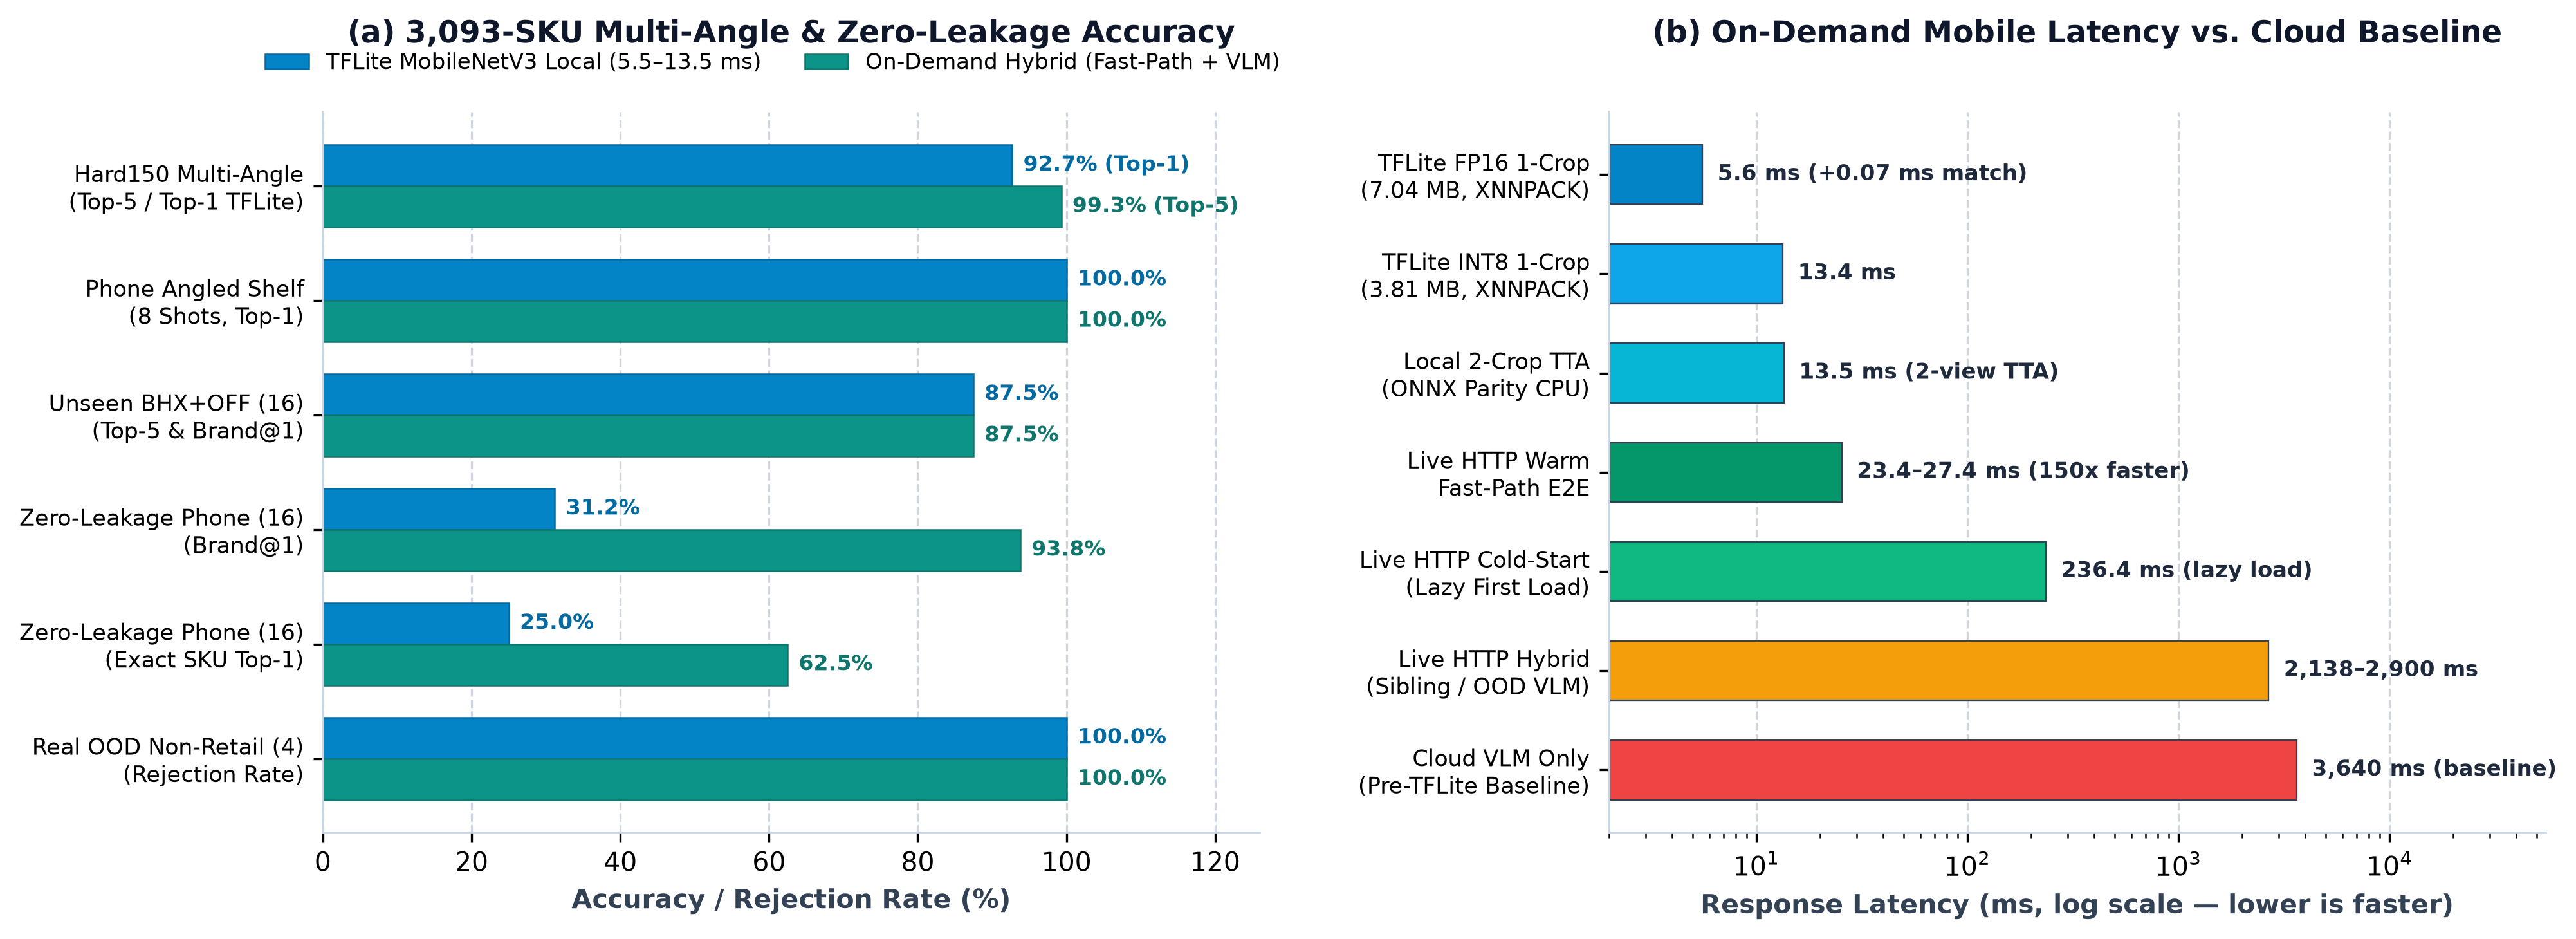
\includegraphics[width=0.98\textwidth]{Images/fig_mobile_tflite_vision.png}
    \caption{3,093-SKU multi-angle and zero-leakage visual recognition accuracy (left) and log-scale on-demand latency comparison of \texttt{MobileNetV3Large-224} TFLite Fast-Path vs.\ cloud VLM baseline (right).}
    \label{fig:mobile_tflite_vision}
\end{figure}

\subsection*{Perishable Forecasting, 50-Store Profit Backtest, and Guard Audits (\texttt{ops\_chest})}
On FreshRetailNet-50K, hourly stockout recovery reduced daily demand WAPE from \textbf{32.3\% to 20.5\%} and virtually eliminated downward bias (\textbf{$-32.3\% \to -0.1\%$}, $n=200{,}000$). Evaluated on 11,037 fully stocked validation points, LightGBM~v3 reduced forecasting WAPE from \textbf{35.1\% (EWMA) to 30.2\%}, reduced bias from \textbf{+6.9\% to +2.7\%}, and achieved \textbf{81\%} empirical coverage for the nominal 80\% prediction interval (vs.\ 73\% for EWMA).

Crucially, however, the 37-day out-of-sample A/B store profit backtest across \textbf{50 held-out stores} (2-fold store CV, Table~\ref{tab:ops_chest_backtest} and Figure~\ref{fig:ops_chest_frn}) demonstrated that lower forecasting WAPE does \emph{not} automatically yield higher retail profit:
\begin{itemize}
    \item Raw \texttt{B-ML} (using LightGBM symmetric interval dispersion) earned only +3.6\% over Baseline~A---\emph{underperforming} \texttt{B-EWMA} (+4.2\%) by $-0.4\%$ median profit and losing $-5.6\%$ on small stores ($\le 30$ SKUs) due to noisy quantile spread inflating perishable waste to 5.7\%.
    \item Asymmetric \texttt{B-ML split} performed even worse (+1.6\% vs.\ A, 6.5\% waste, winning only 6\% of stores against EWMA).
    \item Coupling LightGBM's accurate median ($\hat{q}_{50}$) with EWMA's smooth dispersion ($\sigma_{\text{EWMA}}$) and applying the 2-fold out-of-sample profit gate (\textbf{\texttt{B-Gate}}, \code{size_cut=30}) achieved the best overall performance: \textbf{+4.9\% store profit} over Baseline~A (\textbf{+0.8\%} median gain over \texttt{B-EWMA}, winning on \textbf{76\%} of held-out stores), the \textbf{lowest waste (4.8\%)}, and a \textbf{61\% reduction in top traffic-driver stockouts} (8.7\% $\to$ \textbf{3.4\%}). On Demo Store~18 (164 fresh SKUs), \texttt{B-Gate} achieved +4.5\% profit over Baseline~A.
\end{itemize}

\begin{table}[H]
\centering
\caption{37-day out-of-sample A/B profit backtest across 50 held-out FreshRetailNet-50K stores (2-fold store CV)}
\label{tab:ops_chest_backtest}
\footnotesize
\setlength{\tabcolsep}{4pt}
\begin{tabularx}{\textwidth}{Y r r r r r r}
\toprule
\textbf{Strategy} & \textbf{vs.\ A} & \textbf{vs.\ EWMA} & \textbf{Win\%} & \textbf{Waste\%} & \textbf{OOS\%} & \textbf{Traffic OOS\%} \\
\midrule
Heuristic Baseline A (30\% MD) & 0.0\% & --- & --- & 5.3 & 14.5 & 8.7 \\
\texttt{B-EWMA} (Ops Chest EWMA) & +4.2\% & 0.0\% & --- & 5.2 & 13.6 & 3.9 \\
\texttt{B-ML} (LightGBM \code{sym} $\sigma$) & +3.6\% & $-0.4\%$ & 38\% & 5.7 & 13.1 & 2.7 \\
\texttt{B-ML split} (split-normal $\sigma$) & +1.6\% & $-2.2\%$ & 6\% & 6.5 & \textbf{12.2} & \textbf{2.3} \\
\texttt{B-ML ewma\_sigma} (all SKUs) & +4.5\% & +0.8\% & 74\% & \textbf{4.8} & 14.3 & 3.4 \\
\textbf{\texttt{B-Gate} (Profit-Gated Router)} & \textbf{+4.9\%} & \textbf{+0.8\%} & \textbf{76\%} & \textbf{4.8} & 14.1 & \textbf{3.4} \\
\bottomrule
\end{tabularx}
\end{table}

\begin{figure}[H]
    \centering
    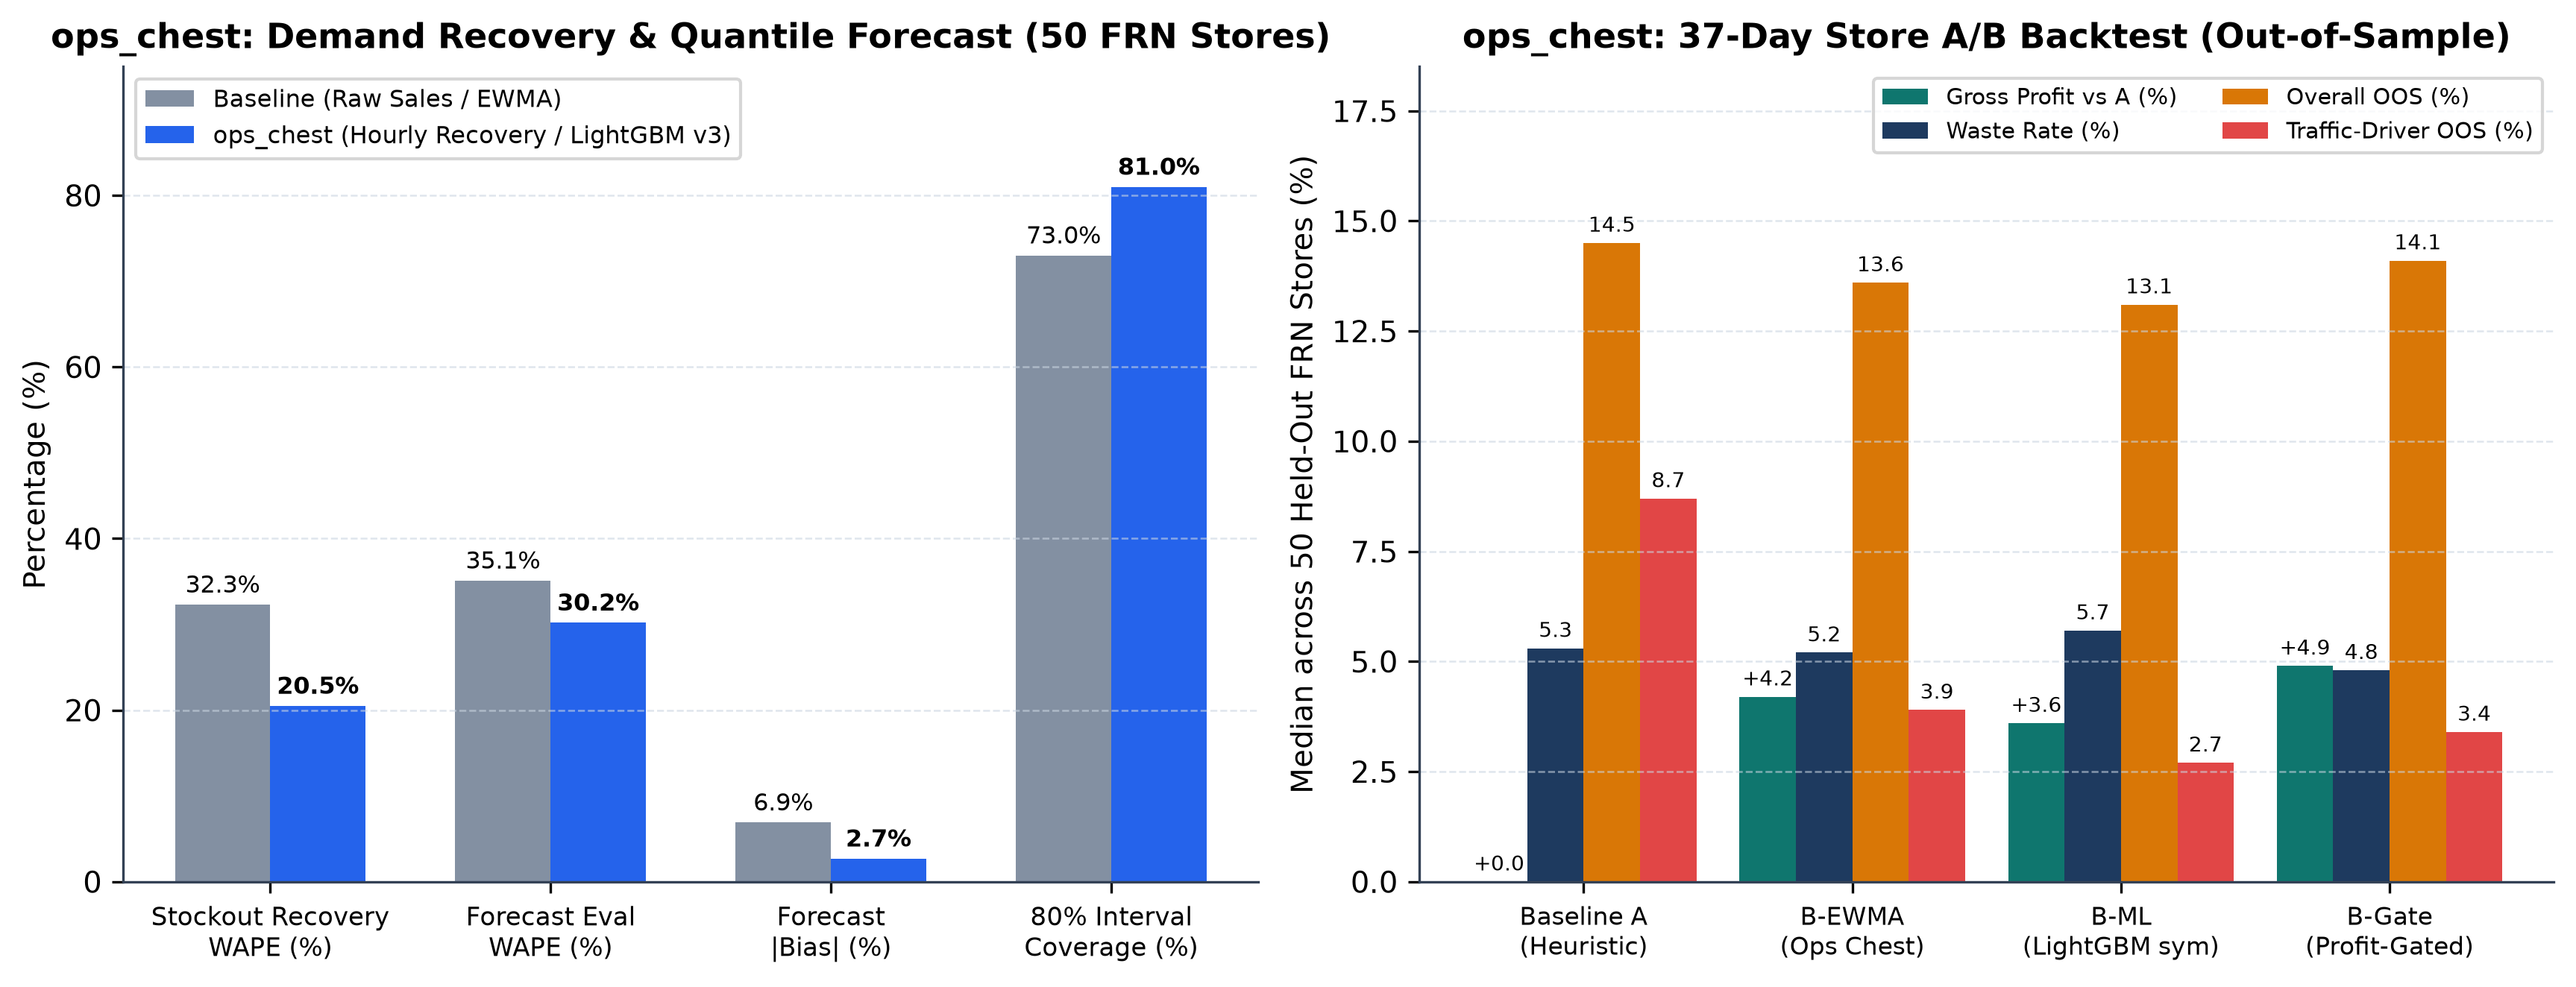
\includegraphics[width=0.98\textwidth]{Images/fig_ops_chest_frn_forecast.png}
    \caption{\texttt{ops\_chest} empirical evaluation on FreshRetailNet-50K: demand recovery and LightGBM~v3 WAPE (left) and 50-store 37-day A/B profit, waste, and stockout comparison (right).}
    \label{fig:ops_chest_frn}
\end{figure}

In parallel, Table~\ref{tab:ops_chest_guard} summarizes the 20-scenario multi-provider runtime failover and grounding evaluation (\code{eval_failover.json}) verifying \texttt{ops\_chest}'s tool-calling reliability and \code{guard.py} enforcement.

\begin{table}[H]
\centering
\caption{\texttt{ops\_chest} runtime tool-calling, grounding, and HITL safety evaluation (\code{eval_failover.json}, $N=20$)}
\label{tab:ops_chest_guard}
\footnotesize
\begin{tabularx}{\textwidth}{L{5.0cm} r r Y}
\toprule
\textbf{Runtime Safety / Quality Metric} & \textbf{Passed} & \textbf{Rate} & \textbf{Verification Scope} \\
\midrule
Numerical Grounding (\code{grounded}) & 20 / 20 & \textbf{100.0\%} & Every number $\ge 1{,}000$ verified in tool output or prompt \\
Correct Tool Selection (\code{tools_ok}) & 19 / 20 & 95.0\% & Appropriate read/proposal tool invoked across 31-tool schema \\
Zero False Execution Claims (\code{no_false_exec}) & 19 / 20 & 95.0\% & Agent must state proposal is \texttt{PENDING}, never auto-executed \\
Strict End-to-End Scenario Pass & 18 / 20 & 90.0\% & All grounding, tool, refusal, and format assertions pass \\
\bottomrule
\end{tabularx}
\end{table}

\section{Qualitative Results}

\subsection*{Live Sales-Floor Voice Kiosk (\texttt{Retail-AI-})}
Figure~\ref{fig:kiosk_live_ui} captures the live \texttt{Retail-AI-} kiosk interface running in Chrome during end-to-end validation, showing the 2D Vietnamese avatar \emph{Mai}, real-time voice controls, grounded recommendation text, and structured Thanh Lam Mart product cards with exact VND prices.

\begin{figure}[H]
    \centering
    \includegraphics[width=0.95\textwidth]{Images/kiosk_live_ui.png}
    \caption{Live desktop \texttt{Retail-AI-} customer voice kiosk interface showing avatar \emph{Mai}, grounded Vietnamese response, and catalog product cards.}
    \label{fig:kiosk_live_ui}
\end{figure}

On mobile viewports ($390\times 844$\,px live at \url{https://mai-retail-kiosk.vercel.app}), Figure~\ref{fig:mobile_popup_live} captures the newly verified \textbf{Product Photo Lightbox Popup} opened after asking \emph{``Tương ớt Chin Su chai 1kg thành phần chính là gì v''} and tapping the rendered product card: the centered overlay frames the full Chin-Su 1\,kg bottle ($299\times 299$\,px on a crisp white canvas), brand/category badges (\texttt{CHIN-SU}, \texttt{Tương Các Loại}), reference price (62,200\,đ/Chai), simulated 30-day sales (284/30 days), quick \emph{``Hỏi thành phần''} action, and dismiss controls with zero layout clipping or console errors.

\begin{figure}[H]
    \centering
    \includegraphics[width=0.42\textwidth]{Images/mobile_product_popup_live.png}
    \caption{Live mobile production capture ($390\times 844$\,px, \url{https://mai-retail-kiosk.vercel.app}) showing the clickable Product Photo Lightbox modal for \emph{Chin Su Chili Sauce 1\,kg} with full packshot, reference pricing, simulated sales badge, and one-tap ingredient prompt.}
    \label{fig:mobile_popup_live}
\end{figure}

Five verified dialogues demonstrate how \texttt{Retail-AI-} handles real supermarket scenarios end-to-end:
\begin{enumerate}
    \item \textbf{Colloquial Bestseller Transparency (\emph{``Ba chỉ bò Mỹ ACEFOODS loại nào bán chạy nhất?''} \& \emph{``cái nào bán chạy nhất v''}):} Rather than fabricating live POS ranks, Mai preserves active category context, strips colloquial Vietnamese particles (\emph{v, vậy, z, nhỉ}), ranks deterministically over \code{demo_sales.sqlite3} ($\approx 212$\,ms), explicitly discloses simulated 30-day provenance, and appends unit-price context.
    \item \textbf{Sub-Second Cost-Feasible Meal Basket (\emph{``Gợi ý bữa tối dưới 150k cho 2 người''}):} Multi-item Path~E backed by Groq LPU \code{fast_chat()} in Singapore (\texttt{sin1}) delivers a complete savory dinner basket with 4 grounded cards inside budget in just \textbf{870\,ms HTTPS} (down from 5.50\,s pre-optimization) with strict \emph{mình/bạn} persona consistency.
    \item \textbf{Quantitative Back-of-Pack Ingredients \& Instant Photo Inspection (\emph{``Tương ớt Chin Su chai 1kg thành phần chính là gì v''}):} Zero-token 3-tier lookup returns exact quantitative ingredients (\emph{``Nước, đường, ớt 110\,g/kg, muối, chất làm dầy (1422), tỏi, cà chua cô đặc...''}) alongside a thumbnail card that opens the full-screen Product Photo Lightbox on tap.
    \item \textbf{Clean Shopper-Facing Zalo Bot Manager Escalation:} Tapping \emph{Gọi quản lý · Zalo} or asking for staff dispatches an immediate Zalo Bot alert to the store manager while showing a polite confirmation without exposing internal UUIDs or raw status enums (\code{NOTIFIED_ZALO}).
    \item \textbf{Clinical Refusal vs.\ Benign Edge Cases:} Queries asking for prescription drugs or disease treatment (\emph{``thuốc hạ sốt trị đau dạ dày''}) trigger an immediate deterministic medical-safety boundary recommending a pharmacist/doctor, whereas benign supermarket queries containing sensitive keywords (XSTest 10/10, e.g., \emph{``nước muối sinh lý súc miệng''} or \emph{``trà gừng uống ấm bụng''}) are answered helpfully without over-refusal.
\end{enumerate}

\subsection*{Store Manager Operations Copilot (\texttt{ops\_chest})}
In back-office walkthroughs on Demo Store~18 (164 fresh SKUs), \texttt{ops\_chest} demonstrates four concrete operational behaviors:
\begin{enumerate}
    \item \textbf{Proactive Morning Briefing \& FEFO Markdown:} Upon querying daily store risks, the agent calls inventory summary and expiring-lot tools, identifies chilled lots within 1--2 days of expiry whose stock exceeds expected full-price sales, calculates graduated markdown prices preserving positive contribution margin, and creates \texttt{PENDING} markdown proposals for one-click manager approval.
    \item \textbf{Vision OCR Shelf Expiry Check:} Uploading a smartphone photo of a fresh-food package triggers \code{vision.py} to extract expiry dates and lot quantities, pre-populating an inline date-check form rather than mutating stock silently.
    \item \textbf{HITL Governance \& Guardrail Interception:} When prompted to ``order 50 packs from supplier X immediately,'' the agent invokes \code{propose_po}, leaves the order in \texttt{PENDING} status, and clearly informs the manager that supplier email dispatch (Mailpit/SMTP) awaits explicit approval; if the LLM attempts to claim execution prematurely, \code{guard.py} catches \code{FALSE_EXEC}.
    \item \textbf{Closed-Loop Hypothesis \& Edit-Habit Learning:} Managers can log operational hypotheses (e.g., weekend rain depressing cold-beverage demand) via \code{propose_hypothesis} for automated post-period verdict scoring (\code{hypotheses.py}), while \code{edit_learning.py} observes recurring manager quantity adjustments to surface bias patterns in future briefings.
\end{enumerate}

\section{Error Analysis and Discussion}

Rigorous failure inspection across both repositories revealed five root causes that shaped the final system design and highlight remaining engineering trade-offs:
\begin{enumerate}
    \item \textbf{Why Lower ML WAPE Lost Store Profit Without a Profit Gate (\texttt{ops\_chest}):} The most instructive empirical finding in \texttt{ops\_chest} is that LightGBM~v3 reduced forecasting WAPE by 4.9 percentage points (35.1\% $\to$ 30.2\%) yet \emph{lost} store profit ($-0.4\%$ median overall, $-5.6\%$ on stores with $\le 30$ SKUs) when its own quantile spread ($q_{90}-q_{10}$) drove Newsvendor safety stock. Because quantile trees trained on short perishable histories over-estimate tail variance on sparse SKUs, replacing LightGBM's dispersion with smooth $\sigma_{\text{EWMA}}$ and gating small stores to EWMA (\texttt{B-Gate}) turned a $-0.4\%$ loss into a \textbf{+0.8\%} profit gain over EWMA (+4.9\% vs.\ Baseline~A).
    \item \textbf{Feature-Shift Failure in Early Forecasting Versions (\texttt{ops\_chest}):} Early LightGBM~v1 included target-day discount as a feature; because future promotions are unknown at forecast time (defaulting to zero), the model systematically under-forecasted by $-15.7\%$. Similarly, v2 price-elasticity deflation ($e \approx 9.6$) induced 14--31\% bias. Removing unobservable future features and anchoring v3 to 56-day EWMA eliminated both biases.
    \item \textbf{Residual 6/100 Strict Failures on Unseen SOTA~V2 Queries (\texttt{Retail-AI-}):} Of the 6 strict failures (4 functional), 2 stem from missing structured allergen/nutrition tables in the Thanh Lam Mart CSV (forcing conservative disclaimers rather than definitive allergen-free guarantees), 2 involve ultra-colloquial regional slang outside catalog aliases, and 2 reflect strict multi-attribute budget phrasing edge cases where exact-unit comparisons require broader pack-size normalization.
    \item \textbf{Fast-Lane Groq LPU vs.\ Cloud Structured JSON Trade-Off (\texttt{Retail-AI-}):} Although tiered Groq LPU streaming + semantic caching + Singapore (\texttt{sin1}) compressed cold single queries to \textbf{508--554\,ms}, $<150\text{k}$ dinner baskets to \textbf{870\,ms}, and cache hits to \textbf{125--140\,ms} at \$0, complex \code{json_schema} edge cases (multi-condition allergy or deep clarification) still route to cloud DeepSeek (1.3--2.0\,s) to stay safely within Groq's free 8k TPM ceiling. On-premise quantized hosting (vLLM) would unify sub-500\,ms latency across both paths.
    \item \textbf{Remaining 2/20 Edge Cases in \texttt{ops\_chest} Failover Evaluation:} In \code{eval_failover.json}, 1 of 20 scenarios missed a secondary read tool under degraded fallback model routing and 1 phrasing border-line triggered a \code{FALSE_EXEC} warning before manager confirmation---reinforcing why structural exclusion of direct-execution tools from the LLM schema remains essential defense-in-depth beyond prompt instructions.
    \item \textbf{Physical Resolution Limit of $224\times 224$ Embeddings on Identical-Layout Pack-Size Siblings (\texttt{Retail-AI-}):} While \texttt{MobileNetV3Large-224} TFLite reached 92.67\% Top-1 on hard multi-angle views and 87.5\% Top-5/Brand@1 on unseen external shots in 5.5--13.5\,ms, $224\times 224$ global embeddings cannot reliably read fine gram/ml typography when two SKUs share identical graphic layouts (e.g., \emph{Tường An 80\,g vs.\ 200\,g} or \emph{TH True Milk unsweetened vs.\ low-sugar}). Introducing the deterministic \emph{Sibling Pack-Size Guard} eliminated false Fast-Path size commits by escalating sibling SKUs to Hybrid VLM while preserving 23--27\,ms instant recognition on visually distinct SKUs.
\end{enumerate}
